\qquad A Tabela \ref{tab:tempos_insertion} apresenta os tempos de execução,
em segundos, obtidos para o Insertion Sort nos seis tamanhos de
instância exigidos pelo trabalho, para cada um dos três tipos de
entrada testados.

\begin{table}[htbp]
    \centering
    \begin{tabular}{|l|r|r|r|r|r|r|}
        \hline
         & 10 & 100 & 1.000 & 10.000 & 100.000 & 1.000.000 \\
        \hline
        Crescente & 0,000001 & 0,000002 & 0,000002 & 0,000016 & 0,000094 & 0,001015 \\
        \hline
        Decrescente & 0,000002 & 0,000003 & 0,000146 & 0,013730 & 1,378020 & 139,297525 \\
        \hline
        Random & 0,000001 & 0,000003 & 0,000076 & 0,007502 & 0,689424 & 69,702984 \\
        \hline
    \end{tabular}
    \caption{Tempo de execução (em segundos) do Insertion Sort por tamanho e tipo de instância}
    \label{tab:tempos_insertion}
\end{table}

\qquad O Gráfico \ref{fig:grafico_insert} apresenta esses mesmos dados em
escala linear. Nele fica evidente que, para tamanhos de até 10.000
elementos, os tempos de execução são praticamente imperceptíveis nas
três situações. A diferença de comportamento só se torna visualmente
clara a partir de 100.000 elementos, quando o tempo das entradas
decrescente e randômica cresce de forma acentuada, enquanto a
entrada crescente permanece próxima de zero.

\begin{figure}[htbp]
    \centering
    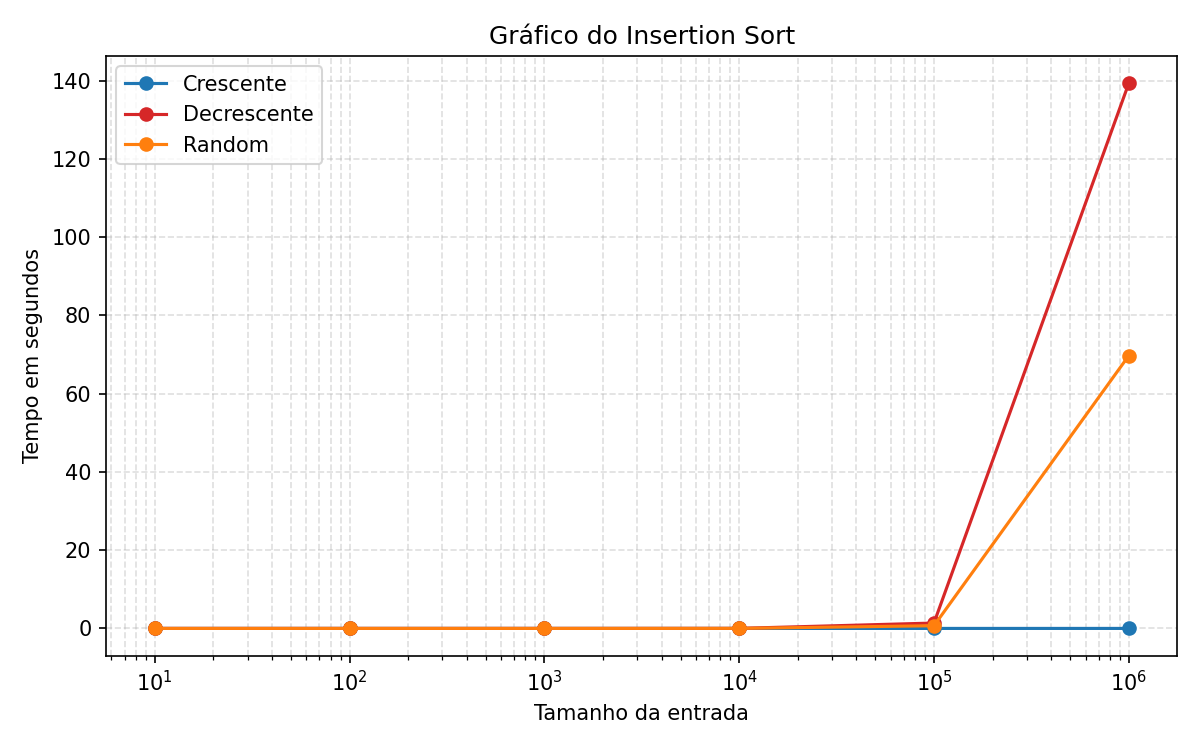
\includegraphics[width=14cm]{Imagens/Insertion Sort/grafico.png}
    \caption{Gráfico de tempo por tamanho do algoritmo Insertion Sort (escala linear)}
    \label{fig:grafico_insert}
\end{figure}

\qquad Como o crescimento quadrático faz com que os valores nas menores
instâncias fiquem visualmente esmagados no gráfico em escala linear,
o Gráfico \ref{fig:grafico_insert_log} apresenta os mesmos dados em
escala logarítmica no eixo do tempo, o que permite observar o
comportamento do algoritmo em todos os tamanhos testados, inclusive
os menores.

\begin{figure}[htbp]
    \centering
    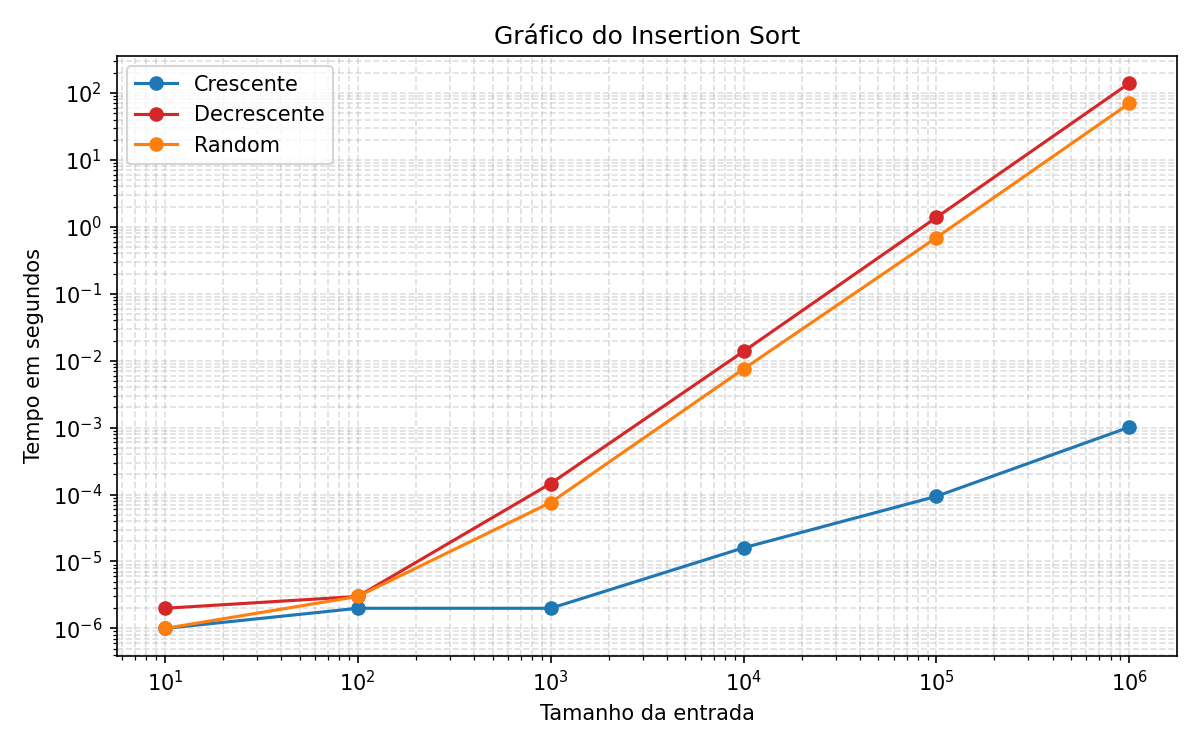
\includegraphics[width=14cm]{Imagens/Insertion Sort/grafico_log.png}
    \caption{Gráfico de tempo por tamanho do algoritmo Insertion Sort (escala logarítmica)}
    \label{fig:grafico_insert_log}
\end{figure}

\qquad Analisando os resultados, observa-se que a entrada crescente
apresenta desempenho linear: mesmo para 1.000.000 de elementos, o
tempo de execução foi de apenas cerca de 0,001 segundo, já que o
laço interno de deslocamento praticamente não é executado quando o
vetor já está ordenado. Já a entrada decrescente, que representa o
pior caso do algoritmo, teve o tempo de execução crescendo de forma
quadrática, chegando a aproximadamente 139,3 segundos para 1.000.000
de elementos. A entrada randômica, representando o caso médio,
também cresceu de forma quadrática, porém com tempo de execução
próximo à metade do pior caso (cerca de 69,7 segundos para 1.000.000
de elementos), o que é compatível com o número esperado de
comparações e deslocamentos em uma entrada aleatória.
